\documentclass[12pt]{article}

% Packages
\usepackage[T1]{fontenc}
\usepackage[margin=1in]{geometry}
\usepackage{amsmath,amssymb}
\usepackage{natbib}
\usepackage{graphicx}
\usepackage{booktabs}
\usepackage{multirow}
\usepackage{longtable}
\usepackage{pdflscape}
\usepackage{xcolor}
\usepackage{hyperref}
\graphicspath{{../../../figures/}}

% Define \subsubsubsection (paragraph-level heading, unnumbered)
\makeatletter
\newcommand{\subsubsubsection}[1]{\paragraph{#1}\mbox{}\par}
\makeatother

% Prefix figure and table numbers with S
\renewcommand{\thefigure}{S\arabic{figure}}
\renewcommand{\thetable}{S\arabic{table}}

\title{Supplementary Materials for:\\SPECTRUM: A Data-Driven, Component-Level Projection Framework for 21st-Century Sea-Level Rise}
\author{Minchew, Meyer, et al.}
\date{}

\begin{document}
\maketitle

\tableofcontents
\clearpage

%% ================================================================
%% MATERIALS AND METHODS
%% ================================================================
\setcounter{secnumdepth}{3}

\section{Materials and Methods}

Unless otherwise noted, all reported intervals are 90\% Bayesian credible intervals (equal-tailed), and where $1\sigma$ is reported (e.g., the rheology correction factor), we state explicitly that it is a standard deviation.




\subsection{Observational datasets}

All component models are calibrated against published observational products (Table~\ref{tab:obs_datasets}). We use:
\begin{itemize}
\item \textbf{Global mean sea level:} NASA satellite altimetry (TOPEX/Jason, 1993--2025; \citealp{Beckley2017,Hamlington2020}), with the Frederikse et~al.~\citeyearpar{Frederikse2020} tide-gauge reconstruction (1900--2018) and the Dangendorf et~al.~\citeyearpar{Dangendorf2024} reconstruction (1900--2021) for pre-satellite validation. None of these records enters any component calibration.
\item \textbf{Ocean thermal expansion:} NOAA thermosteric sea level (doi:10.7289/V53F4MVP), 0--700\,m (1955--2025) and 0--2000\,m (2005--2025) \citep{Levitus2012}. Both records are scaled by a factor of 1.14 before fitting. \citet{Li2022} show that linear vertical interpolation between standard depth levels cannot reproduce the curvature of the temperature--depth profile at the vertical resolution of the historical data, and that replacing it with a multiply-rotated piecewise cubic Hermite scheme raises the 1956--2020 upper-ocean (0--700\,db) thermosteric trend from 0.48 to 0.55\,mm\,yr$^{-1}$, an increase of 14\%. The uncorrected NOAA 0--700\,m trend over 1955--2025 is 0.49\,mm\,yr$^{-1}$, close to their linearly interpolated estimate, and the scaling raises it to 0.55\,mm\,yr$^{-1}$, matching their value for the cubic scheme. A residual structural uncertainty of 5\% of the corrected signal is retained after the scaling. \citet{Li2022} attribute most of the bias to the sparser vertical sampling of the pre-1990 record, so a uniform scaling reproduces their corrected trend over the full record while also raising the post-1990 rate by 14\%. The 700--2000\,m layer is carried by the 0--2000\,m record from 2005 onward and by the deep layer of the two-layer model at earlier times. A constant $0.07 \pm 0.04$~mm\,yr$^{-1}$ \citep{Purkey2010, Desbruyeres2016} is added over the full record for the contribution below 2000\,m.
\item \textbf{Glaciers:} GlaMBIE global consensus (The GlaMBIE Team~\citeyear{GlaMBIE2025}), combining glaciological field measurements, satellite altimetry, DEM differencing, and GRACE/GRACE-FO gravimetry across all 19 RGI regions. We use 2000--2023 (23 annual points) for calibration.
\item \textbf{Greenland:} Mouginot et~al.~\citeyearpar{Mouginot2019} SMB and discharge (1972--2018), of which the 44 years from 1975 enter the discharge fit, the earlier years being excluded because the lagged ocean forcing is undefined before then. Mankoff et~al.~\citeyearpar{Mankoff2021} discharge (1986--2023) and the IMBIE-3 Greenland record (1972--2023; Otosaka et~al.~\citeyear{Otosaka2026}) are withheld for validation. Subsurface ocean temperature from EN4 v4.2.2 with g10 bias corrections (200--500\,m, Greenland peripheral waters, 1970--2021; Good et~al.~\citeyear{Good2013}). Surface temperature from Berkeley Earth \citep{Rohde2020}.
\item \textbf{Antarctica:} IMBIE-3 mass balance (1979--2023, 45 annual points per region; Otosaka et~al.~\citeyear{Otosaka2026}), partitioned into West Antarctica, East Antarctica, and the Antarctic Peninsula.
\item \textbf{Terrestrial water storage:} Frederikse et~al.~\citeyearpar{Frederikse2020} reconstruction, used only from 2003 onward, the period over which it derives from GRACE and GRACE-FO observations rather than from process models.
\item \textbf{Temperature scenarios:} IPCC AR6 assessed GMST projections (SSP1-2.6, SSP2-4.5, SSP3-7.0, SSP5-8.5; \citealp{Lee2021}).
\end{itemize}

\begin{table}[ht]
\centering
\caption{Datasets used in the component framework and the role each plays. Records marked \emph{validation} are withheld from every component calibration, including observed GMSL itself. Parenthetical counts are the annual points that enter the corresponding calibration likelihood. A complete dataset inventory including versions, spatial domains, and processing details is provided in \texttt{data/dataset\_inventory.xlsx}.}
\label{tab:obs_datasets}
\footnotesize
\setlength{\tabcolsep}{3pt}
\begin{tabular}{lllll}
\toprule
Component & Dataset & Span & Role & Reference \\
\midrule
GMSL & NASA altimetry & 1993--2025 & Validation & Beckley et~al.~\citeyearpar{Beckley2017} \\
GMSL & Frederikse reconstruction & 1900--2018 & Validation & Frederikse et~al.~\citeyearpar{Frederikse2020} \\
GMSL & Dangendorf reconstruction & 1900--2021 & Validation & Dangendorf et~al.~\citeyearpar{Dangendorf2024} \\
\midrule
Thermosteric & NOAA thermosteric, 0--700\,m & 1955--2025 (71) & Calibration & Levitus et~al.~\citeyearpar{Levitus2012} \\
Thermosteric & NOAA thermosteric, 0--2000\,m & 2005--2025 (21) & Calibration & Levitus et~al.~\citeyearpar{Levitus2012} \\
Thermosteric & Frederikse steric & 1900--2018 & Validation & Frederikse et~al.~\citeyearpar{Frederikse2020} \\
\midrule
Glaciers & GlaMBIE global consensus & 2000--2023 (23) & Calibration & The GlaMBIE Team~\citeyearpar{GlaMBIE2025} \\
\midrule
Greenland & Mouginot discharge \& SMB & 1972--2018 (44) & Calibration & Mouginot et~al.~\citeyearpar{Mouginot2019} \\
Greenland & EN4 subsurface ocean T & 1970--2021 & Forcing & Good et~al.~\citeyearpar{Good2013} \\
Greenland & Mankoff PROMICE discharge & 1986--2023 & Validation & Mankoff et~al.~\citeyearpar{Mankoff2021} \\
Greenland & IMBIE-3 Greenland & 1972--2023 & Validation & Otosaka et~al.~\citeyearpar{Otosaka2026} \\
\midrule
Peninsula & IMBIE-3 Peninsula & 1979--2023 (45) & Calibration & Otosaka et~al.~\citeyearpar{Otosaka2026} \\
EAIS & IMBIE-3 East Antarctica & 1979--2023 (45) & Diagnostic & Otosaka et~al.~\citeyearpar{Otosaka2026} \\
WAIS & IMBIE-3 West Antarctica & 1979--2023 (45) & Calibration & Otosaka et~al.~\citeyearpar{Otosaka2026} \\
\midrule
TWS & Frederikse TWS (GRACE era) & 2003--2018 & Forcing & Frederikse et~al.~\citeyearpar{Frederikse2020} \\
\midrule
Temperature & Berkeley Earth surface T & 1850--2024 & Forcing & Rohde \& Hausfather~\citeyearpar{Rohde2020} \\
Temperature & IPCC AR6 GMST projections & 2015--2099 & Forcing & Lee et~al.~\citeyearpar{Lee2021} \\
Projections & IPCC AR6 FACTS & 2020--2150 & Comparison & Garner et~al.~\citeyearpar{Garner2023} \\
\bottomrule
\end{tabular}
\end{table}

\subsection{Component model posteriors}
\label{s:component_posteriors}

This section collects the parameter posteriors of every calibrated component model. Greenland discharge is fitted by weighted least squares over a discrete set of delays, so its posterior is a mixture of normals weighted by the Bayesian Information Criterion and is shown as marginal densities. The remaining components are sampled by Markov chain Monte Carlo and are shown as corner plots, with marginal histograms on the diagonal and pairwise joint densities off it, so that the parameter trade-offs the marginals hide can be read directly. The fitted values quoted in the captions are the posterior medians with their 90\% credible intervals, and they are the values carried into the projections.

\begin{figure}[ht]
\centering
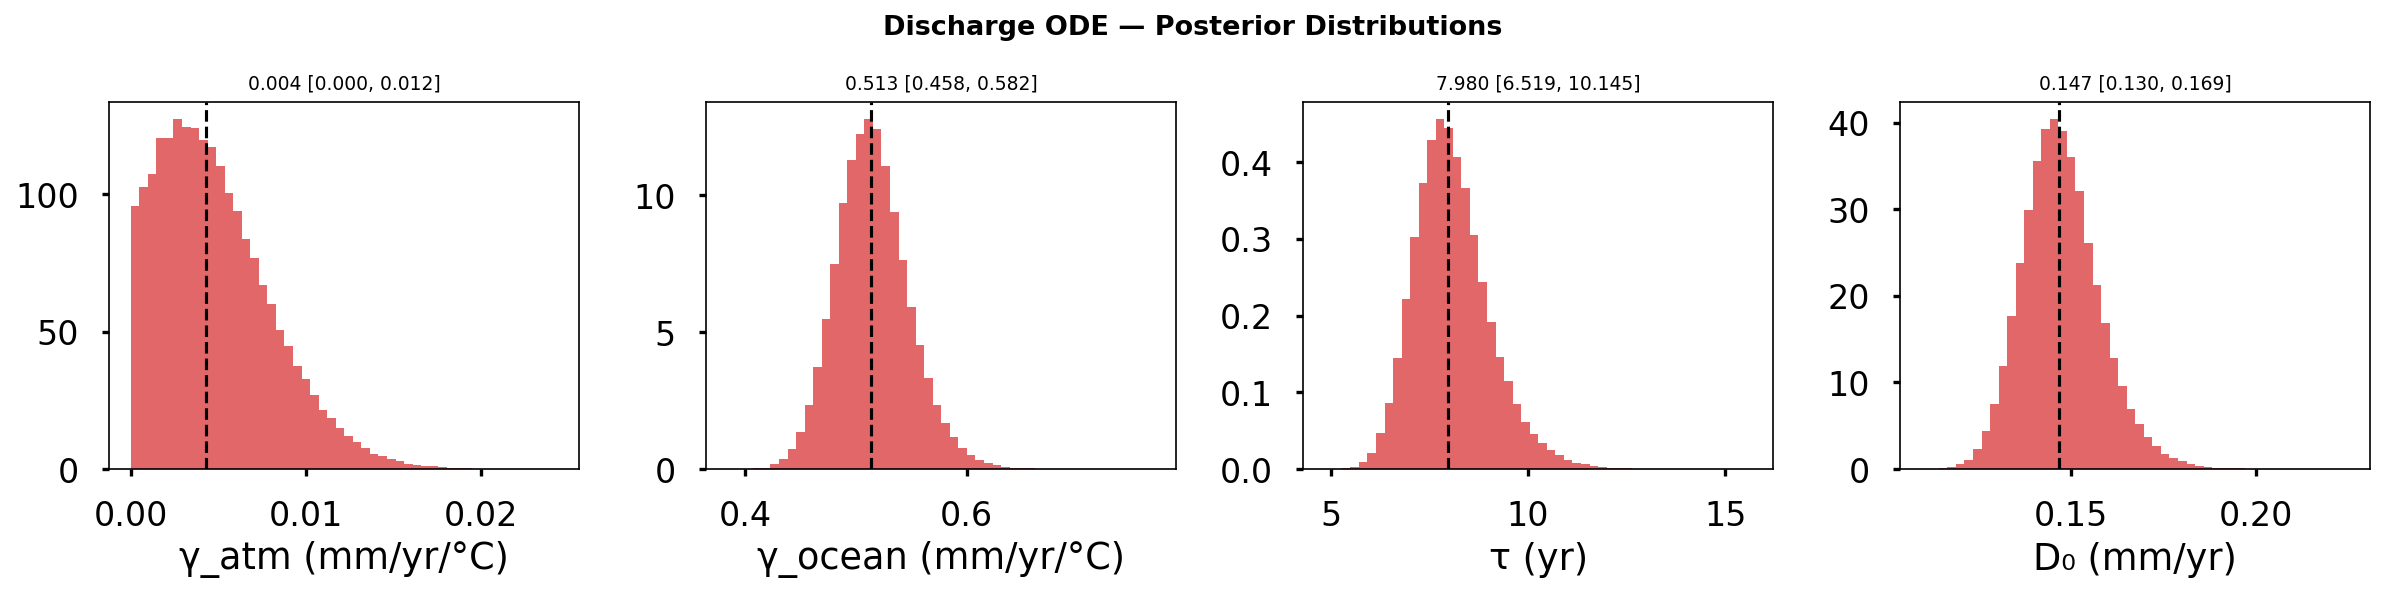
\includegraphics[width=\textwidth]{component_greenland_discharge_posteriors.png}
\caption{\textbf{Greenland discharge delay model parameter posteriors.} Marginal posteriors for the three parameters of the discharge delay model calibrated against \citet{Mouginot2019}. \textbf{(a)} The sensitivity of discharge to cumulative delayed ocean thermal forcing, $\gamma$, and \textbf{(b)} the background discharge rate, $r_0$. Both are shown as the exact marginal density, a mixture of normals over the candidate delays weighted by the Bayesian Information Criterion, rather than as a histogram of posterior draws. Dashed lines mark the posterior median and dotted lines the 5th and 95th percentiles. \textbf{(c)} The delay $\delta$ is resolved only to integer years, so its posterior is the set of weights over the candidate delays, which place 99.5\% of the weight on $\delta = 5$\,yr. Panel titles give the median with the 90\% credible interval.}
\label{fig:greenland_discharge_posteriors}
\end{figure}

\begin{figure}[ht]
\centering
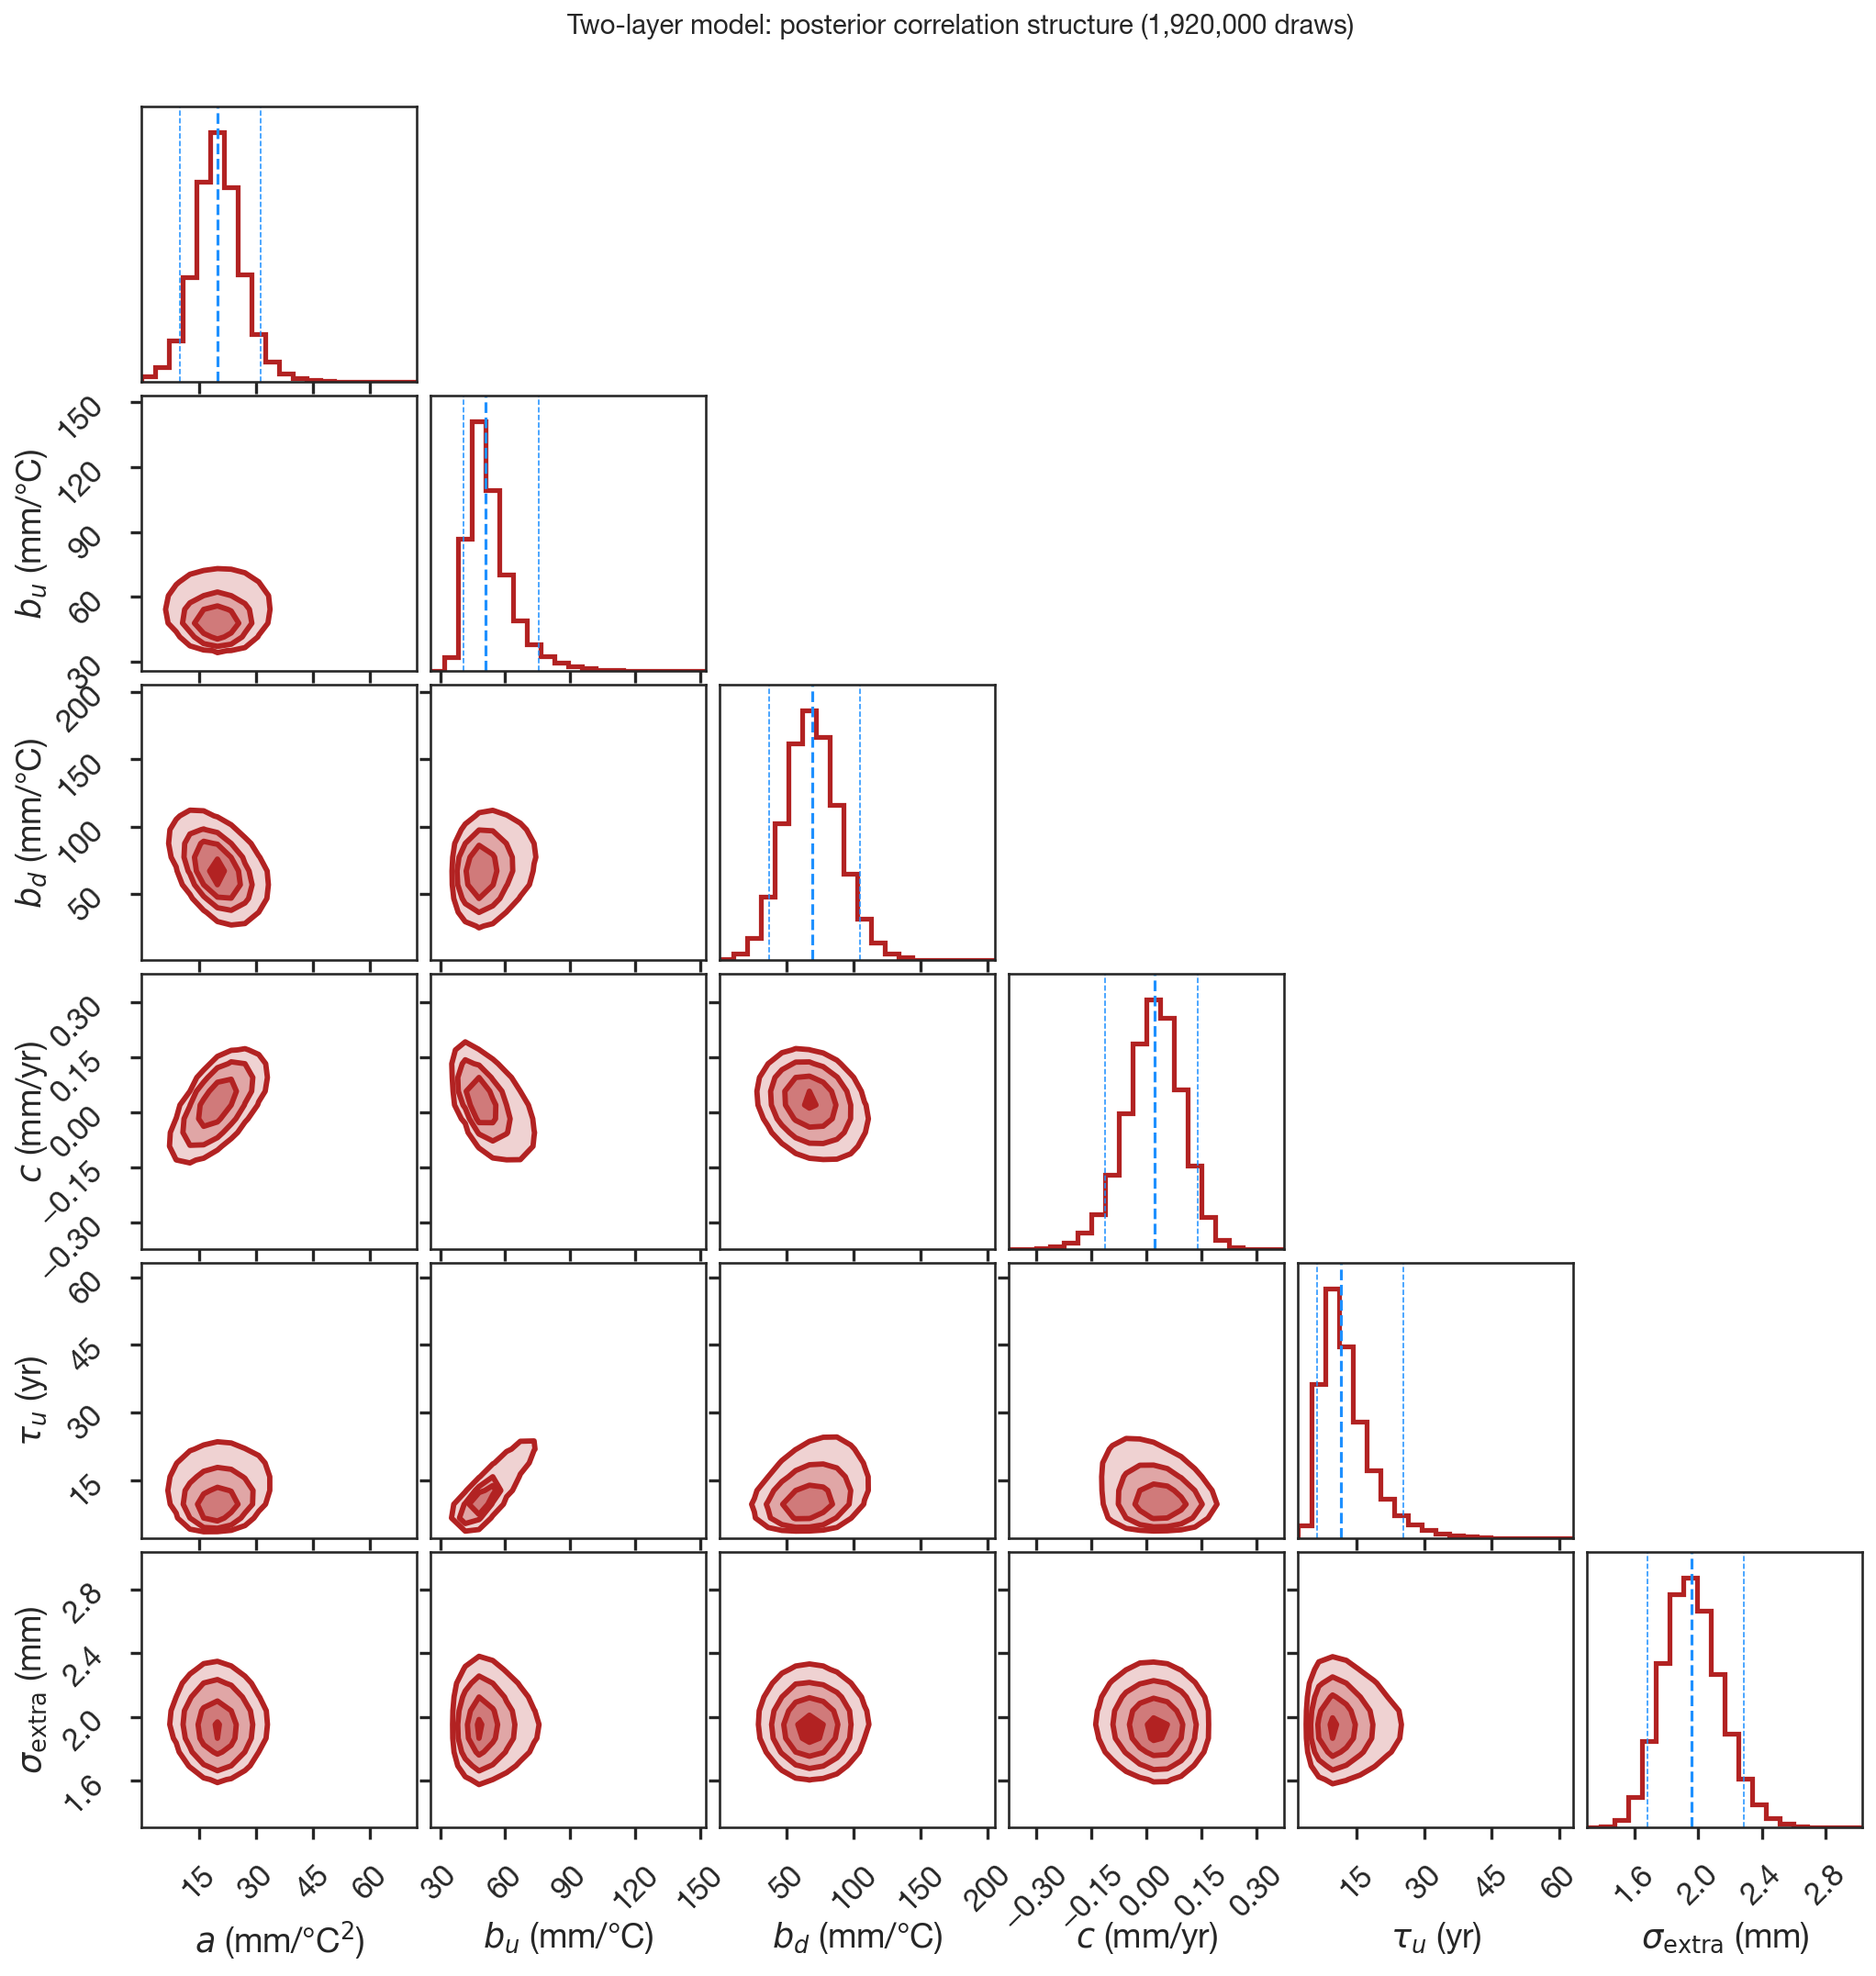
\includegraphics[width=0.9\textwidth]{component_ocean_posterior_corner.png}
\caption{\textbf{Two-layer thermosteric model posterior correlation structure.} The joint posterior for the six parameters of the two-layer energy balance model fitted to NOAA 0--700\,m and 0--2000\,m thermosteric sea level data. Diagonal panels show marginal posterior histograms (red), with dashed vertical lines marking the median and 90\% credible interval. Off-diagonal panels show the joint posterior density, with contours denoting 1, 2, and 3 standard deviations. Only $\tau_u$ has an informative prior (black curve) while the other five parameters have flat, uninformative priors (not shown).}
\label{fig:ocean_priors_posteriors}
\end{figure}



\begin{figure}[ht]
\centering
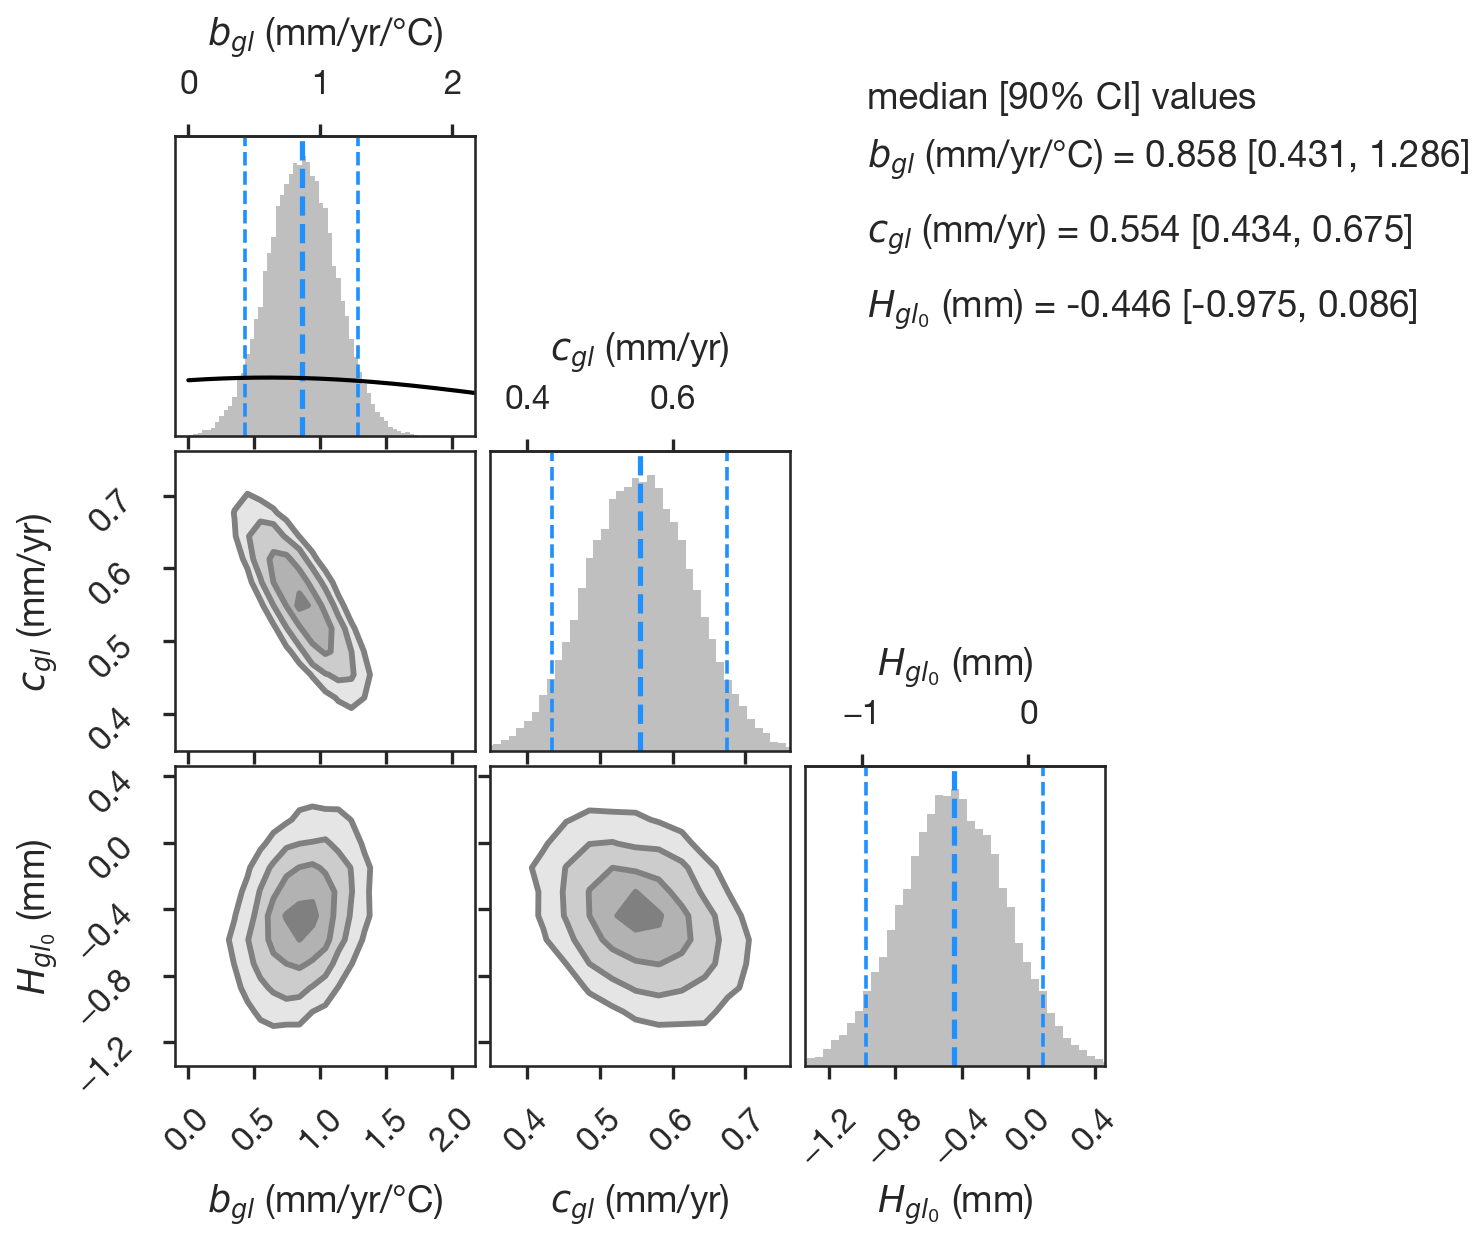
\includegraphics[width=0.9\textwidth]{component_glacier_posterior_corner.png}
\caption{\textbf{Glacier model posterior correlation structure.} The joint posterior for the three parameters of the glacier model, the warming sensitivity $b_{gl}$, the committed rate $c_{gl}$, and the baseline offset $H_{gl_0}$, fitted to the GlaMBIE record \citep{GlaMBIE2025} with the full covariance of the cumulative record in the likelihood. Diagonal panels show marginal posterior histograms, with dashed vertical lines marking the median and the 5th and 95th percentiles. Off-diagonal panels show the joint posterior density, with contours denoting 1, 2, and 3 standard deviations. Posterior medians are $b_{gl} = 0.745$ mm yr$^{-1}$ $^\circ$C$^{-1}$ [0.297, 1.201], $c_{gl} = 0.574$ mm yr$^{-1}$ [0.452, 0.695], and $H_{gl_0} = -0.490$ mm [$-1.011$, 0.045], where brackets give 90\% credible intervals. Only $b_{gl}$ carries an informative prior (black curve), centered on the sensitivity of \citet{Rounce2023} and wide enough that the posterior is set by the data. The slope and intercept of a common record, $b_{gl}$ and $c_{gl}$, are strongly anti-correlated, whereas $H_{gl_0}$ is only weakly correlated with either because the temperature integral is anchored at the year 2000 baseline rather than at the start of the temperature record.}
\label{fig:glacier_corner}
\end{figure}

\begin{figure}[ht]
\centering
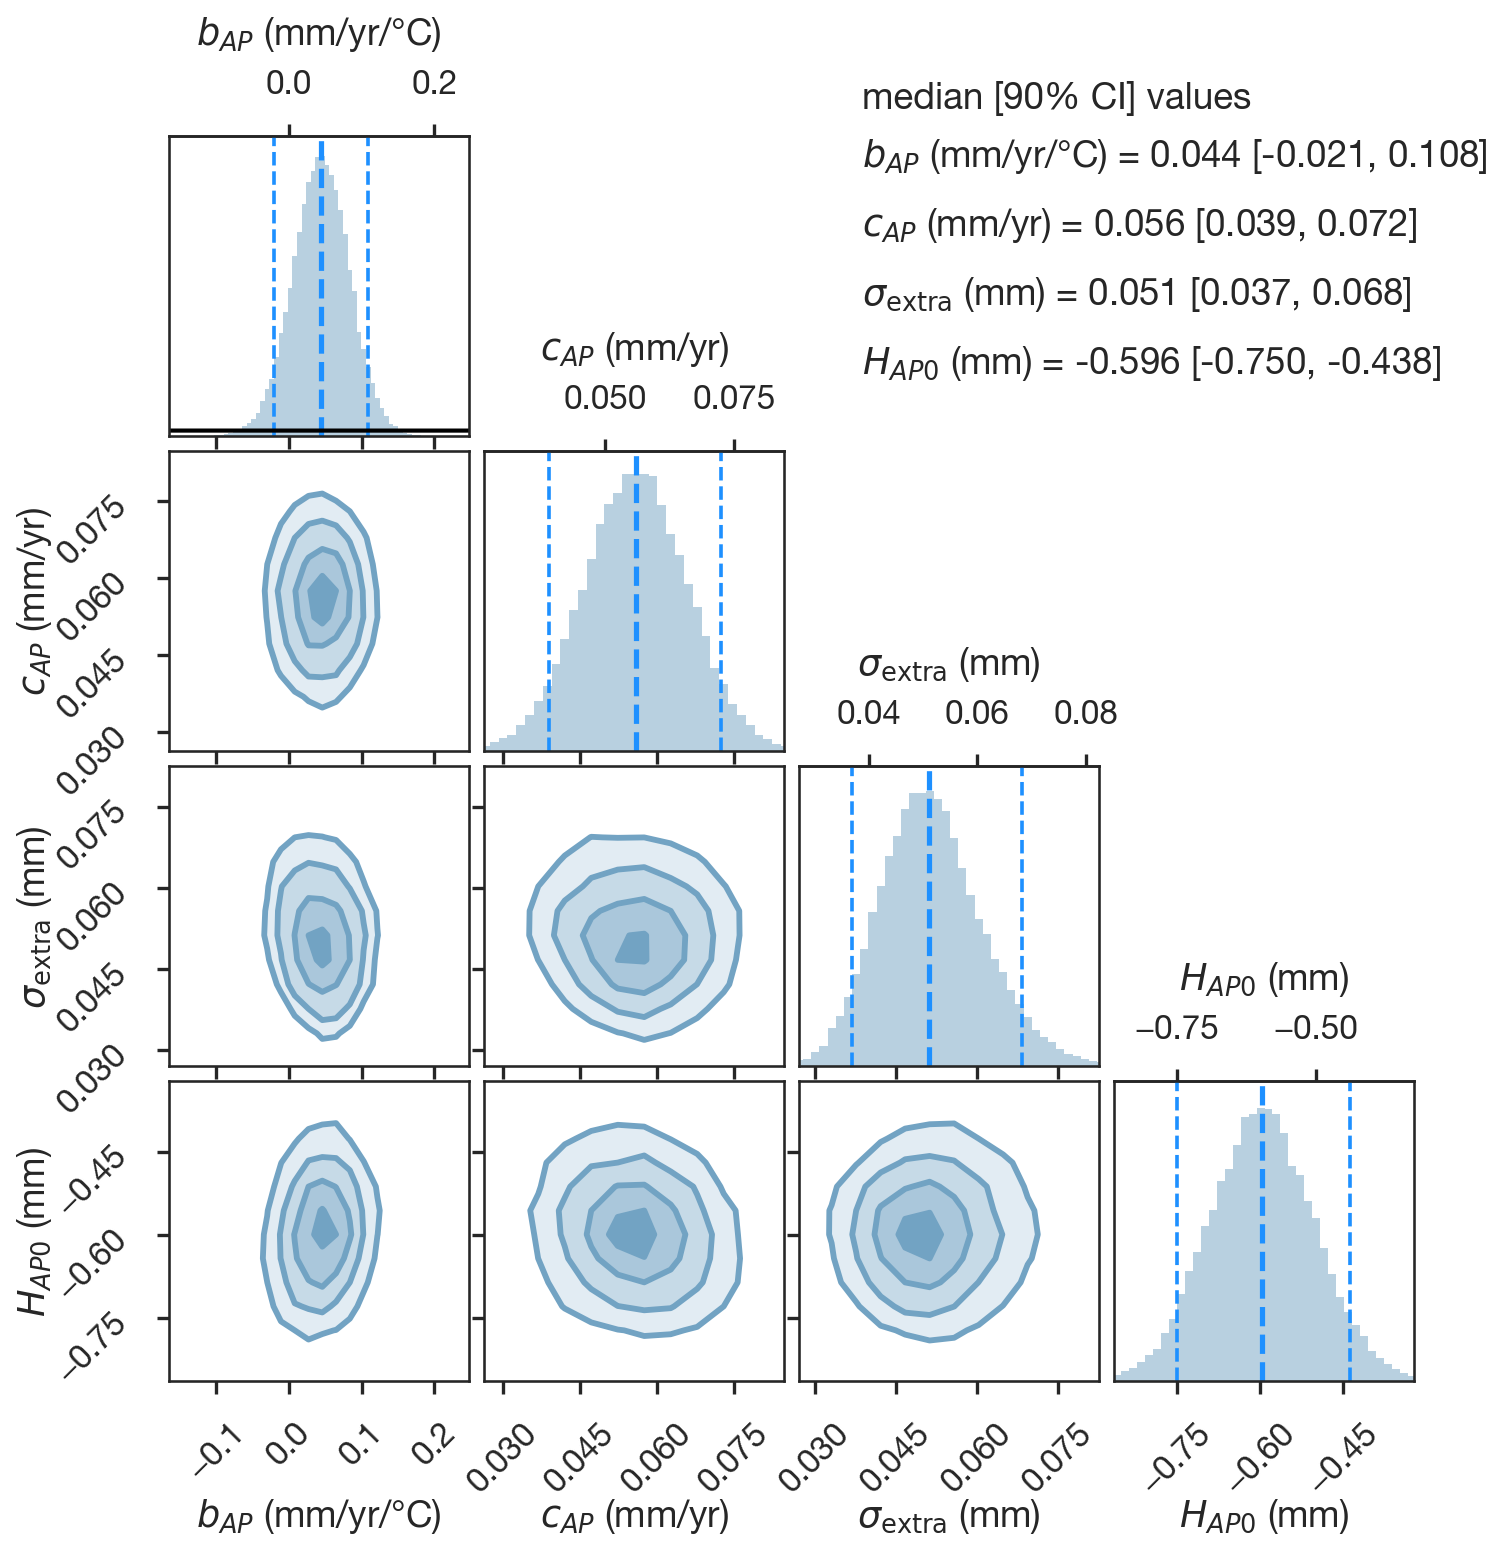
\includegraphics[width=0.9\textwidth]{component_apeninsula_posterior_corner.png}
\caption{\textbf{Antarctic Peninsula model posterior correlation structure.} The joint posterior for the four parameters of the Peninsula model, the warming sensitivity $b_{AP}$, the committed rate $c_{AP}$, the model-inadequacy term $\sigma_{\mathrm{extra}}$, and the baseline offset $H_{AP0}$, fitted to the IMBIE-3 Peninsula record \citep{Otosaka2026} with the full covariance of the cumulative record in the likelihood. Diagonal panels show marginal posterior histograms, with dashed vertical lines marking the median and the 5th and 95th percentiles. Off-diagonal panels show the joint posterior density, with contours denoting 1, 2, and 3 standard deviations. Posterior medians are $b_{AP} = 0.044$ mm yr$^{-1}$ $^\circ$C$^{-1}$ [$-0.021$, 0.108], $c_{AP} = 0.056$ mm yr$^{-1}$ [0.039, 0.072], $\sigma_{\mathrm{extra}} = 0.051$ mm [0.037, 0.068], and $H_{AP0} = -0.596$ mm [$-0.750$, $-0.438$], where brackets give 90\% credible intervals. The prior on $b_{AP}$ (black curve) is flat over the range the data support. The credible interval on $b_{AP}$ spans zero, so the record does not resolve the sign of the temperature sensitivity, while the committed rate $c_{AP}$ is well separated from zero. The posterior for $\sigma_{\mathrm{extra}}$ is likewise well separated from zero, confirming that the IMBIE-3 Peninsula record carries annual scatter beyond its reported uncertainty. All four parameters are close to mutually independent, the near-circular off-diagonal contours showing that the excess-noise term absorbs scatter without trading off against the fitted rate--temperature relationship.}
\label{fig:peninsula_corner}
\end{figure}

\begin{figure}[ht]
\centering
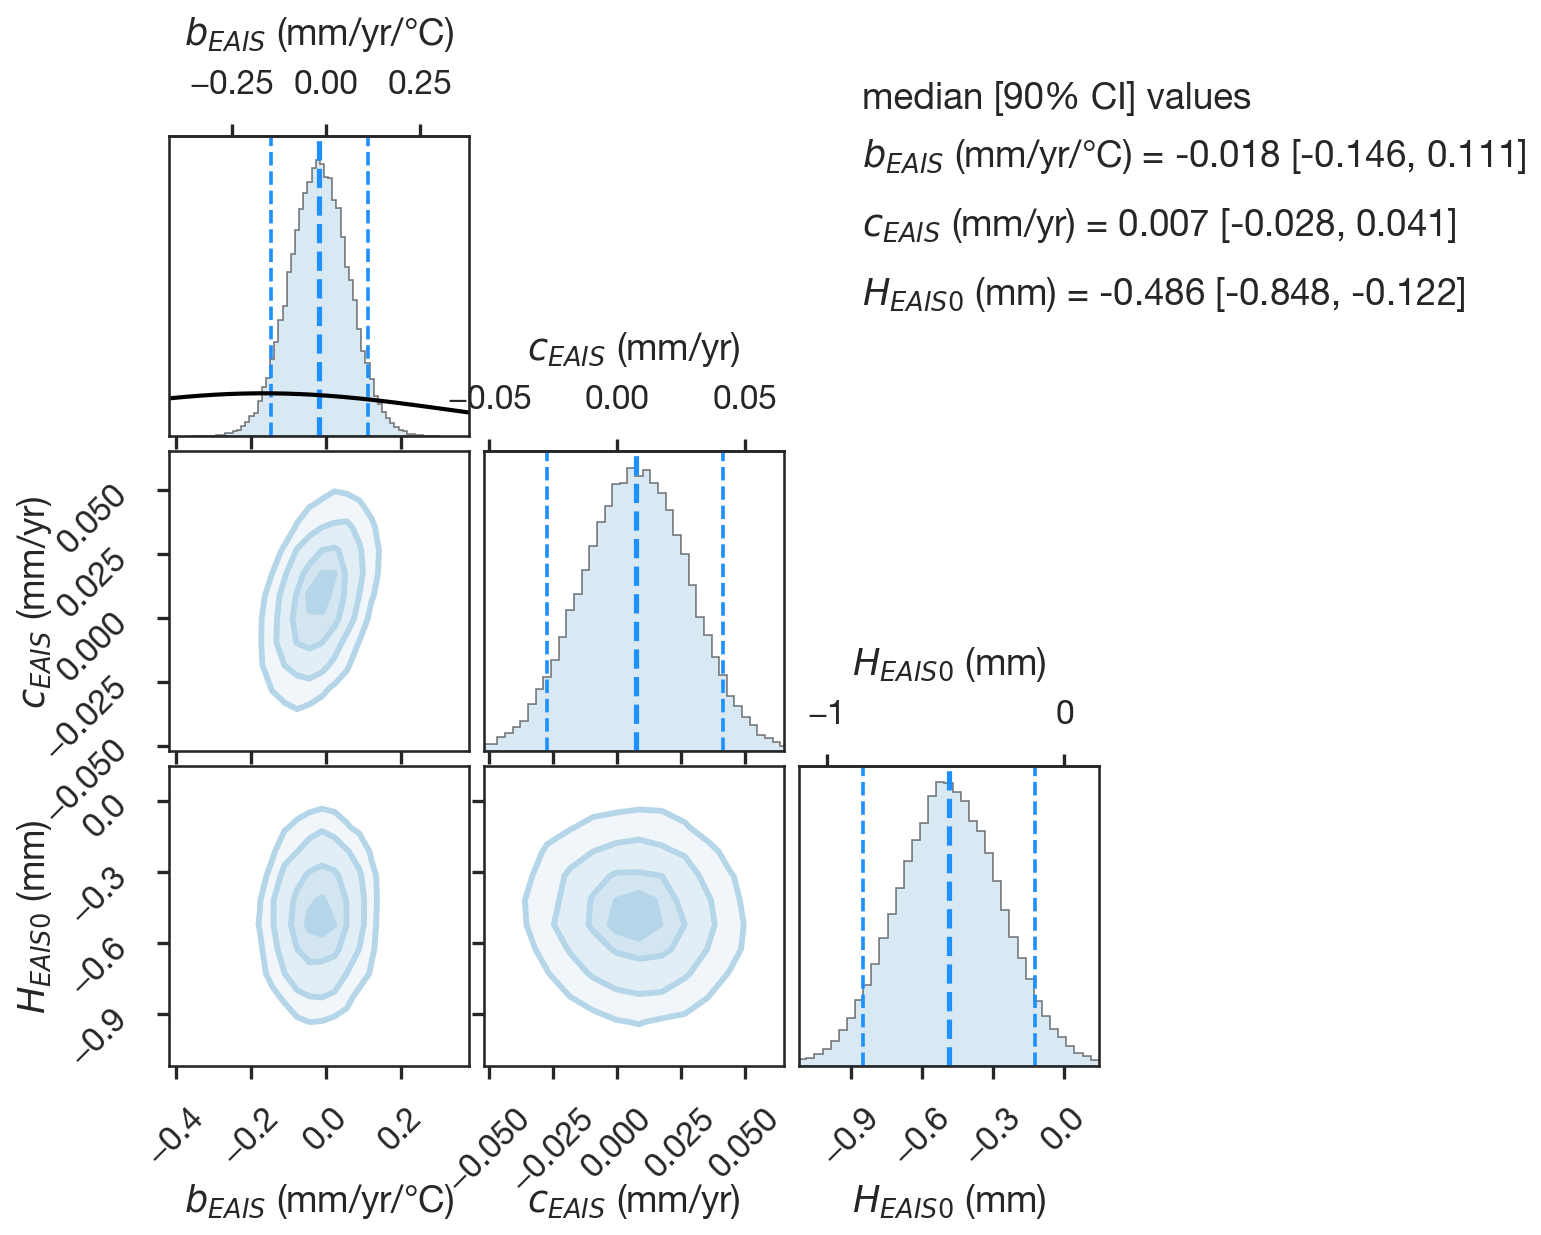
\includegraphics[width=0.9\textwidth]{component_eais_posterior_corner.png}
\caption{\textbf{EAIS model posterior correlation structure.} The joint posterior for the three parameters of the East Antarctic model, the warming sensitivity $b_{EAIS}$, the committed rate $c_{EAIS}$, and the baseline offset $H_{EAIS0}$, fitted to the IMBIE-3 East Antarctic record \citep{Otosaka2026} with the full covariance of the cumulative record in the likelihood. Diagonal panels show marginal posterior histograms, with dashed vertical lines marking the median and the 5th and 95th percentiles. Off-diagonal panels show the joint posterior density, with contours denoting 1, 2, and 3 standard deviations. Posterior medians are $b_{EAIS} = -0.015$ mm yr$^{-1}$ $^\circ$C$^{-1}$ [$-0.145$, 0.111], $c_{EAIS} = 0.007$ mm yr$^{-1}$ [$-0.027$, 0.041], and $H_{EAIS0} = -0.480$ mm [$-0.846$, $-0.114$], where brackets give 90\% credible intervals. Only $b_{EAIS}$ carries an informative prior (black curve), which is wide enough that the posterior is set by the data. Both the sensitivity and the committed rate have credible intervals spanning zero, consistent with an ice sheet close to balance over the IMBIE-3 record, which is why this fit serves as a diagnostic and the projection instead adopts the literature surface-mass-balance sensitivity $C_T = 60 \pm 20$~Gt\,yr$^{-1}$\,$^\circ$C$^{-1}$ \citep{Frieler2015,Ligtenberg2013}. The posterior is correspondingly uninformative in its correlation structure as well, with $b_{EAIS}$ and $c_{EAIS}$ weakly positively correlated and $H_{EAIS0}$ nearly independent of both.}
\label{fig:eais_corner}
\end{figure}

\subsection{Variance decomposition}

A variance decomposition using the law of total variance across the three policy-relevant SSPs (1-2.6, 2-4.5, 3-7.0) attributes 90\% of total forecast variance to within-scenario uncertainty---predominantly WAIS (88\% of total variance)---and 10\% to between-scenario differences. Cross-component covariances are small ($+0.0006$~m$^2$, representing 0.3\% of total variance), confirming that the independent calibration approach does not introduce material correlations.

\subsection{Temperature scenarios}



%% ================================================================
\subsection{Component-level skill metrics}

Table~\ref{tab:skill_metrics} collects the goodness-of-fit statistics for every component fitted to data. We report reduced chi-square rather than a coefficient of determination. Every component is calibrated against a cumulative record whose variance is dominated by its trend, so $R^2$ in that space approaches unity for any model that reproduces the trend at all and says little about the quality of the fit. A straight line in time, with no temperature dependence whatsoever, scores 0.983 against the 0--2000\,m thermosteric record.

Reduced chi-square compares the residuals with the uncertainty the calibration data are reported to carry, so a value near unity indicates both that the model reproduces the observations to within their stated errors and that the error model used in the likelihood is well specified. The normalization is not identical in every case, and we note where it differs. Glaciers, the Antarctic Peninsula, and EAIS are fitted to cumulative records whose errors are serially correlated, and their $\chi^2$ is therefore evaluated against the full covariance of the cumulative record built from the reported annual uncertainties, not against a diagonal approximation, which would understate the residual scatter that the reported errors can absorb. All three sit between 0.91 and 1.04. The Peninsula reaches that value only with a fitted model-inadequacy term $\sigma_{p,\mathrm{extra}}$, described in the Antarctic Peninsula section of the main text. Without it the reduced chi-square is 2.64, so the IMBIE-3 Peninsula record carries real annual scatter beyond its reported per-year uncertainty. Glaciers and EAIS need no such term. For the thermosteric model the quoted value includes the fitted excess-noise term $\sigma_{\mathrm{extra}}$ in the point variance and is normalized by the number of data points rather than by the degrees of freedom, so it sits slightly below the corresponding $\chi^2/\mathrm{dof}$. The 0--2000 m value of 0.36 indicates that the 21-year record is fitted to well inside its reported error rather than that the fit is poor. The Greenland discharge value of 1.83 is the generalized chi-square of the demeaned cumulative fit before the error scale is recalibrated. It is the quantity by which the parameter covariance is subsequently inflated, so it is a statement about the reported errors being too small rather than about the model missing the data. Its degrees of freedom are 41, being the 44 fitted points less one for the demeaning of the cumulative record and two for the fitted parameters. The \citet{Mouginot2019} discharge record runs from 1972, but the delayed ocean forcing is undefined before 1975 because EN4 begins in 1970 and the selected lag is 5\,yr, so the first three years of the discharge record do not enter the fit.

Two components need further comment. WAIS is fitted in time rather than in temperature, so no statistic comparable with the other rows is available for it. A weighted least-squares cross-check on the same record, using diagonal rather than correlated weights, gives $\chi^2 = 22.9$ on 45 annual points with three free parameters, and favors a cubic in time over the quadratic by $\Delta\mathrm{BIC} = -4.5$. We retain the quadratic because the purpose of the WAIS fit is to set the starting rate and acceleration for the Scenario 1 extrapolation rather than to identify the polynomial order best supported by a 45-year record, and a cubic extrapolated to 2100 is governed by a term the observations constrain only weakly. EAIS is listed as a diagnostic because the East Antarctic Ice Sheet is close to balance over the IMBIE-3 record, leaving little signal for a temperature-dependent model to recover. The fit is consistent with the reported errors, but the projection adopts a literature surface-mass-balance sensitivity, $C_T = 60 \pm 20$~Gt\,yr$^{-1}$\,$^\circ$C$^{-1}$ \citep{Frieler2015,Ligtenberg2013}, and uses the regression only as a check on that value.

One further fit enters the framework without being a component model in its own right. The linear surface-to-ocean transfer function given in the main text, which carries SSP temperature trajectories into the Greenland discharge model, explains a modest fraction of the interannual variance, $R^2 = 0.38$ over 52 common annual values, with a residual standard deviation of 0.20\,$^\circ$C that is propagated into the projections. It is the weakest statistical link in the Greenland projection chain, and it is retained rather than replaced because the quantity it must supply is the multi-decadal trend in subsurface temperature rather than its year-to-year variability. Greenland SMB, by contrast, is not fitted. It is passed through as RACMO observations over the historical period and projected with literature sensitivities drawn from the spread between regional climate models \citep{Fettweis2020,Noel2021,Glaude2024}, so no skill metric attaches to it.

These are all within-sample statistics, and on their own they establish only that each model is consistent with the record it was fitted to. The tests that bear on forecasting skill are out of sample. The thermosteric model is compared against the \citet{Frederikse2020} steric reconstruction, withheld from calibration, with an RMS difference of 2.5\,mm over 1957--2018 and 3.8\,mm before 1957, where that reconstruction is itself constrained by models rather than by subsurface observations. Greenland discharge is compared against the \citet{Mankoff2021} record (1986--2023) and the IMBIE-3 time series \citep{Otosaka2026}, neither of which enters the fit. The model falls within error of both for discharge and for total mass balance. As noted in the main text, the \citet{Mankoff2021} comparison is the weaker of the two, because that record shares its underlying raw data with the \citet{Mouginot2019} calibration and differs from it in processing rather than in provenance. IMBIE-3 is the more informative test, being a combination of independent mass-balance estimates from satellite observations of ice flow, surface elevation, and gravimetry. The WAIS quadratic reaches 8.8 $\pm$ 0.7\,mm at 2024 against the IMBIE-3 value of 9.0 $\pm$ 0.7\,mm. The tests that exercise the framework as a whole rather than one component at a time are budget closure, in which the summed components are compared with satellite altimetry that no component calibration saw, and the hindcast of the level, rate, and transient sensitivity of GMSL since 1950. Both are presented in the Results of the main text.

\begin{table}[h]
\centering
\caption{Goodness-of-fit for the component models fitted to data. For glaciers, the Peninsula, and EAIS, $\chi^2/\mathrm{dof}$ is evaluated against the full covariance of the cumulative record. For the thermosteric model it is normalized by the number of data points rather than by the degrees of freedom and includes the fitted $\sigma_{\mathrm{extra}}$ in the point variance. For Greenland discharge it is the generalized chi-square before error-scale recalibration. Dataset references are given in Table~\ref{tab:obs_datasets}. Greenland SMB and terrestrial water storage are not calibrated against data and are omitted.}
\label{tab:skill_metrics}
\footnotesize
\setlength{\tabcolsep}{4.5pt}
\begin{tabular}{llcl}
\toprule
Component & Calibration data & Reduced $\chi^2$ & Model \\
\midrule
Thermosteric (0--700\,m)  & NOAA, 1955--2025 (71)     & 1.12 & Two-layer, 6 fitted \\
Thermosteric (0--2000\,m) & NOAA, 2005--2025 (21)     & 0.36 & Joint with 0--700\,m \\
Glaciers                  & GlaMBIE, 2000--2023 (23)  & 1.04 & Linear rate--$T$ \\
Greenland discharge       & Mouginot, 1975--2018 (44) & 1.83 & Delay, 2 fitted \\
Antarctic Peninsula       & IMBIE-3, 1979--2023 (45)  & 0.98 & Linear rate--$T$ \\
EAIS (diagnostic)         & IMBIE-3, 1979--2023 (45)  & 0.91 & Linear rate--$T$ \\
WAIS                      & IMBIE-3, 1979--2023 (45)  & ---  & Quadratic in time \\
\bottomrule
\end{tabular}
\end{table}

%% ================================================================
\section{Exceedance Probability by Threshold and Scenario}
\label{sec:exceedance_table}
%% ================================================================

Table~\ref{tab:exceedance} reports the probability of exceeding selected global mean sea-level thresholds (relative to pre-industrial) by 2100 under three warming trajectories, for the full component forecast (which includes the WAIS scenario mixture) and the slow-WAIS scenario alone. Together these columns isolate the contribution of WAIS tail risk: any probability present in the component forecast but absent in the slow-WAIS column is attributable to the possibility of rapid WAIS retreat.

\begin{table}[h!]
\centering
\caption{\textbf{Probability (\%) of exceeding global mean sea-level thresholds by 2100.} Thresholds are relative to the pre-industrial baseline ($\approx$1850--1900). The component forecast column reflects the full WAIS scenario mixture; the slow-WAIS column conditions on the stable-retreat scenario only. Values are computed from posterior samples under each warming trajectory.}
\label{tab:exceedance}
\begin{tabular}{cl rr}
\hline
\textbf{SLR threshold} & \textbf{Warming} & \textbf{Component} & \textbf{Slow} \\
\textbf{(m, pre-ind.)} & \textbf{trajectory} & \textbf{forecast} & \textbf{WAIS} \\
\hline
\multirow{3}{*}{0.5}  & 2\,$^\circ$C & 100.0 & 100.0 \\
                       & 3\,$^\circ$C & 100.0 & 100.0 \\
                       & 4\,$^\circ$C & 100.0 & 100.0 \\
\hline
\multirow{3}{*}{0.75} & 2\,$^\circ$C &  85.5 &   1.3 \\
                       & 3\,$^\circ$C & 100.0 &  98.9 \\
                       & 4\,$^\circ$C & 100.0 & 100.0 \\
\hline
\multirow{3}{*}{1.0}  & 2\,$^\circ$C &  39.6 &   0.0 \\
                       & 3\,$^\circ$C &  70.5 &   0.1 \\
                       & 4\,$^\circ$C &  97.7 &  76.8 \\
\hline
\multirow{3}{*}{1.5}  & 2\,$^\circ$C &  10.1 &   0.0 \\
                       & 3\,$^\circ$C &  15.3 &   0.0 \\
                       & 4\,$^\circ$C &  27.2 &   0.0 \\
\hline
\multirow{3}{*}{2.0}  & 2\,$^\circ$C &   3.4 &   0.0 \\
                       & 3\,$^\circ$C &   4.5 &   0.0 \\
                       & 4\,$^\circ$C &   7.5 &   0.0 \\
\hline
\end{tabular}
\end{table}

%% ================================================================
\section{Value of Information Analysis}
\label{sec:voi}
%% ================================================================

The value of information (VoI) analysis quantifies the economic benefit of resolving the binary uncertainty about whether WAIS retreat remains slow (Scenario 1) or allows for the possibility of rapid retreat (Scenario 2). The framework follows the expected value of sample information (EVSI) formulation from classical decision theory \citep{Raiffa1961}.

\subsection{Decision framework}

We consider an illustrative coastal adaptation decision where a planner must choose a defense height $d$ (meters of sea-level protection) to minimize total expected costs, evaluated against the sea-level rise distribution $S$ at a representative target year of 2100. For a given sea-level rise distribution $S$ at 2100, the total annual cost of defense height $d$ is
\begin{equation}
C(d) = C_{\mathrm{adapt}}(d) + \mathbb{E}\bigl[D\bigl(\max(S - d,\, 0)\bigr)\bigr],
\label{eq:total_cost}
\end{equation}
where $C_{\mathrm{adapt}}(d) = c_a \cdot d$ is the annualized adaptation cost and $\mathbb{E}\bigl[D(\cdot)\bigr]$ is the expected value of the residual damage $D$ from SLR exceeding the defense height (overtopping).

\subsubsection{Adaptation cost}
\label{s:adaptation_cost}

The total capital cost of coastal adaptation is estimated at $C_{\mathrm{cap}} = \$4$\,T/m of GMSLR. This is derived from Tiggeloven et~al.~\citeyearpar{Tiggeloven2020}, who estimate that 3.4\% of the global coastline ($\sim$54{,}400~km of $\sim$1.6~million~km total) warrants dike heightening under cost-benefit optimality, at a unit cost of \$7\,M per km per meter of dike height (the median cost raising dikes in New Orleans post-Hurricane Katrina). This yields $\sim$\$400\,B/m for dike raising alone along the optimal 3.4\% of coastline. We apply a conservative 10$\times$ multiplier to account for the full societal adaptation burden---including seawalls, nature-based solutions, managed retreat, and infrastructure relocation---across a broader fraction of the global coastline.

Because the cost function $C(d)$ (Eq.~\ref{eq:total_cost}) combines adaptation costs with annual flood damages from Jevrejeva et~al.~\citeyearpar{Jevrejeva2018}, both terms need to be expressed in consistent units. Adaptation is dominated by capital investment deployed over the planning horizon, so we conservatively annualize $C_{\mathrm{cap}}$ using the capital recovery factor (CRF):
\begin{equation}
c_a = C_{\mathrm{cap}} \times \mathrm{CRF}, \qquad \mathrm{CRF} = \frac{r\,(1+r)^n}{(1+r)^n - 1},
\label{eq:crf}
\end{equation}
where $r = 0.03$ is the real discount rate and $n = 75$\,yr is the planning horizon. This gives $\mathrm{CRF} \approx 0.034$ and an annualized adaptation cost of $c_a \approx \$135$\,B/(m$\cdot$yr)of GMSLR. The resulting $C(d)$ is in \$/yr, the EVSI is in \$/yr, and the NPV conversion (Eq.~\ref{eq:voi}) produces a present-value total in \$.

\subsubsection{Damage function}

Residual flood damages are computed using the piecewise-linear global damage function of Jevrejeva et~al.~\citeyearpar{Jevrejeva2018}, which maps SLR to annual global flood costs based on estimated asset exposure. For SLR beyond the tabulated range (1.80~m), we extrapolate linearly using the slope of the final segment ($\sim$\$13.8\,T/yr per meter).

\subsection{Two-world structure}

The forecast distribution is decomposed into two conditional distributions, conditioned directly on A4 scenario membership rather than on a percentile-threshold proxy:
\begin{itemize}
\item \textbf{Slow WAIS} ($S_{\mathrm{slow}}$) samples from the blended forecast conditional on WAIS Scenario 1 (\texttt{S1\_status\_quo}) representing future GMSLR.
\item \textbf{Fast WAIS} ($S_{\mathrm{fast}}$) samples from the full forecast conditional on WAIS Scenario 2 (\texttt{S2\_fast\_wais}), representing outcomes that allow for rapid WAIS retreat via MISI, with or without MICI.
\end{itemize}
Because the A4 framework now comprises exactly these two scenarios, $S_{\mathrm{slow}}$ and $S_{\mathrm{fast}}$ partition the full mixture completely: every Monte Carlo sample's WAIS scenario assignment is recorded at the point of sampling and carried through the component-summation and rate-space-blending pipeline as a per-sample label, so the two-world split is exact rather than approximate.

The current prior probability of stable WAIS is $p_s = 0.10$, consistent with our scenario weights (Scenario~1 receives 10\% probability).

\subsection{EVSI calculation}

For a given prior $p_s = P(\text{slow WAIS})$, the EVSI quantifies the annual benefit of learning whether WAIS will lose mass slowly or rapidly before choosing the defense height for coastal development.

\subsubsection{Hedging cost (no information)}

Without additional information, the planner hedges by choosing the single defense height $d^*_{\mathrm{hedge}}$ that minimizes the prior-weighted expected cost:
\begin{equation}
C^*_{\mathrm{hedge}} = \min_{d}\; \bigl[\, p_s \cdot C_{\mathrm{slow}}(d) + (1 - p_s) \cdot C_{\mathrm{fast}}(d) \,\bigr],
\label{eq:hedge}
\end{equation}
where $C_{\mathrm{slow}}(d) = C_{\mathrm{adapt}}(d) + \mathbb{E}[D(\max(S_{\mathrm{slow}} - d, 0))]$ and $C_{\mathrm{fast}}(d)$ is defined analogously using $S_{\mathrm{fast}}$.

\subsubsection{Perfect information cost}

With perfect information, the planner would tailor the defense height to whichever world is realized:
\begin{equation}
C^*_{\mathrm{perfect}} = p_s \cdot \min_{d}\, C_{\mathrm{slow}}(d) \;+\; (1 - p_s) \cdot \min_{d}\, C_{\mathrm{fast}}(d).
\label{eq:perfect}
\end{equation}

\subsubsection{Annual EVSI}

The annual value of perfect information is the difference between the hedging cost and the perfect-information cost:
\begin{equation}
\mathrm{EVSI}_{\mathrm{ann}} = \max\bigl(C^*_{\mathrm{hedge}} - C^*_{\mathrm{perfect}},\; 0\bigr).
\label{eq:evsi}
\end{equation}
This is the annual cost penalty of having to compromise on a single design rather than tailoring to the true state. When $p_s \approx 0$ or $p_s \approx 1$, the hedging design is already close to the tailored design, so EVSI is small. EVSI is maximized near $p_s \approx 0.5$, where the optimal designs for the two worlds diverge most.

\subsection{Discounting and the VoI surface}

The annual EVSI is converted to a net present value (NPV) by discounting the stream of benefits from the year information arrives ($t_a$) to the target year ($t_T = 2100$) at a real discount rate $r = 3\%$:
\begin{equation}
\mathrm{VoI}(t_a, p_s) = \mathrm{EVSI}_{\mathrm{ann}}(p_s)\left( \frac{1 - (1+r)^{-(t_T - t_a)}}{r}\right).
\label{eq:voi}
\end{equation}
The annuity factor $[1 - (1+r)^{-n}]/r$ captures the number of discounted years over which the improved decision yields benefits.

The VoI surface (Fig.~4c of the main text) is computed over a grid of arrival years ($t_a \in [2026, 2150]$) and prior probabilities ($p_s \in [0.01, 0.99]$). All calculations use the 3$\,^\circ$C (SSP2-4.5) warming trajectory. The choice of warming trajectory has qualitatively little impact on the results given all the uncertainties involved. Note that our cost estimates are likely to be underestimates (see \S\ref{s:adaptation_cost}), but the takeaway message remains even if the true costs or damages are an order of magnitude lower. 

\subsection{Key assumptions and limitations}

The VoI calculation is intended to be simple analysis to make a simple point, not to stand for detailed financial decisions. As such, we make several simplifying assumptions:
\begin{enumerate}
\item \textbf{Binary resolution.} Information perfectly resolves the slow/fast dichotomy. Partial information (e.g., updating $p_s$ from 0.10 to 0.30 without full resolution) would yield lower VoI.
\item \textbf{Single decision.} The planner makes one irreversible design choice. In practice, adaptive management with staged decisions would reduce the hedging penalty, lowering VoI.
\item \textbf{Global aggregation.} Costs are aggregated globally. Local VoI would differ based on coastal exposure and elevation.
\item \textbf{Linear adaptation cost.} We assume $C_{\mathrm{adapt}}$ scales linearly with defense height. Economies or diseconomies of scale would modify the optimal designs.
\item \textbf{Discount rate.} The 3\% real discount rate is standard for infrastructure but lower rates (reflecting intergenerational equity) would increase VoI. Higher discount rates, that would lower VoI, are unlikely given the long timeline of risk exposure from sea level rise. 
\end{enumerate}

Despite these simplifications, the analysis provides a rough order-of-magnitude estimate of the economic value of resolving WAIS uncertainty, supporting the argument that targeted investment in ice-sheet observations and process understanding has massive expected returns.



%% ================================================================
%% REFERENCES
%% ================================================================

\bibliographystyle{agufull08}
\bibliography{references}

\end{document}